\documentclass[10pt]{article}
\usepackage{amsfonts} 

\usepackage[T1]{fontenc}
\usepackage[latin1]{inputenc}
%\usepackage{beton}
%\usepackage{ccfonts}
%\usepackage{concrete}
\usepackage{concmath}
\usepackage{eulervm}
\usepackage{amsmath,amsthm,amssymb}
\usepackage{mathtools}
\usepackage{multicol}
\usepackage{marginnote}
\usepackage{pgfplots}
\usepackage{float}
\usepackage{hyperref}
\pgfplotsset{compat=1.5}
\usepackage{graphicx}
\graphicspath{ {./images/} }
\usepackage{listings}
\usepackage{xcolor}
\definecolor{codegreen}{rgb}{0,0.6,0}
\definecolor{codegray}{rgb}{0.5,0.5,0.5}
\definecolor{codepurple}{rgb}{0.58,0,0.82}
\definecolor{backcolour}{rgb}{0.95,0.95,0.92}
\lstdefinestyle{mystyle}{
    backgroundcolor=\color{backcolour},   
    commentstyle=\color{codegreen},
    keywordstyle=\color{magenta},
    numberstyle=\tiny\color{codegray},
    stringstyle=\color{codepurple},
    basicstyle=\ttfamily\footnotesize,
    breakatwhitespace=false,         
    breaklines=true,                 
    captionpos=b,                    
    keepspaces=true,                 
    numbers=left,                    
    numbersep=5pt,                  
    showspaces=false,                
    showstringspaces=false,
    showtabs=false,                  
    tabsize=2
}

\lstset{style=mystyle}

\usepackage{mathtools}

\usepackage{wasysym}
\usepackage[margin=1.5in]{geometry} 
\usepackage{enumerate}
\index{\usepackage}\usepackage{multicol}

\newcommand{\N}{\mathbf{N}}
\newcommand{\Z}{\mathbb{Z}}

\newcommand{\R}{\mathbf{R}}
\newcommand{\C}{\mathbf{C}}
\newcommand{\Pbb}{\mathbb{P}}
\newcommand{\Fcal}{\mathcal{F}}
\newcommand{\Acal}{\mathcal{A}}
\newcommand{\Ecal}{\mathcal{E}}
\newcommand{\Ebb}{\mathbb{E}}
\newcommand{\Qbb}{\mathbb{Q}}

\newenvironment{theorem}[2][Theorem]{\begin{trivlist}
  \item[\hskip \labelsep {\bfseries #1}\hskip \labelsep {\bfseries #2.}]}{\end{trivlist}}
\newenvironment{lemma}[2][Lemma]{\begin{trivlist}
  \item[\hskip \labelsep {\bfseries #1}\hskip \labelsep {\bfseries #2.}]}{\end{trivlist}}
\newenvironment{exercise}[2][Exercise]{\begin{trivlist}
  \item[\hskip \labelsep {\bfseries #1}\hskip \labelsep {\bfseries #2.}]}{\end{trivlist}}
\newenvironment{reflection}[2][Reflection]{\begin{trivlist}
  \item[\hskip \labelsep {\bfseries #1}\hskip \labelsep {\bfseries #2.}]}{\end{trivlist}}
\newenvironment{proposition}[2][Proposition]{\begin{trivlist}
  \item[\hskip \labelsep {\bfseries #1}\hskip \labelsep {\bfseries #2.}]}{\end{trivlist}}
\newenvironment{corollary}[2][Corollary]{\begin{trivlist}
  \item[\hskip \labelsep {\bfseries #1}\hskip \labelsep {\bfseries #2.}]}{\end{trivlist}}

\newenvironment{definition}[2][Definition]{\begin{trivlist}
  \item[\hskip \labelsep {\bfseries #1}\hskip \labelsep {\bfseries #2.}]}{\end{trivlist}}

\begin{document}
	
  \renewcommand{\qedsymbol}{\smiley}
	\title{Non linear feature extraction of the stratosphere \\ Summary}
	\author{Marijn van der Meer}
	\maketitle

\section{Introduction}
In the two hemispheres of the Earth, the atmosphere over the polar regions is shaped into a vortex of winds, culminating in mid-winter. Every two years, on average, a surge of warming in the stratosphere, e.g. the second layer of the atmosphere as you go upward after the troposphere,  disrupts the 
wind field resulting in vortex distortions. As explained in~\cite{Sigmond2013}, expertise in seasonal forecasting in extratropical regions is relatively lacking. This encourages the seasonal forecast community to look for further sources of predictability. The authors of~\cite{Sigmond2013} propose that insight into the state of the stratosphere can act as a source of increased seasonal predictability because long-term circulation anomalies in the lower stratosphere that follow sudden stratospheric warming are related to circulation anomalies in the troposphere, e.g. the lowest layer of Earth's atmosphere, that may last up to two months. Thus,  sudden stratospheric warming (SSW) impacts strongly the weather at the Earth's surface up to three months following their appearance~\cite{Baldwin581} and exploiting these events could produce improved long term forecasts. 

\section{Data.}

The variability of the vortex is studied using the Potential Vorticity (PV). This measures the absolute circulation of a packet of air enclosed between two isentropic surfaces. It is applied in atmospheric dynamics and meteorology to describe rotating fluids with vertical stratification. PV values in the troposphere are generally low. Yet, potential vorticity increases rapidly from the troposphere to the stratosphere due to the substantial shift in static stability. 
Our PV data at 850K was sourced in the northern-hemisphere (latitiude > 30\textdegree) from ERA-Interim reanalysis during October to April every six hours from 1979 to 2018. This yields 33960 time snapshots of potential vorticity. Furthermore, the data covers a regular longitude/latitude grid with 0.75\textdegree spacing, yielding 38880 grid cells. An illustration of the potential vorticity (disturbed and undisturbed) can be seen in Fig.~\ref{fig:example_vortex}. \newline

Three datasets are provided: 
\begin{enumerate}
    \item Basis: 38400 rows for 1002 dimensions, latitude and longitude also provided \\
    \item Raw data: 33960 for 1002 dimensions\\
    \item Anomalies data: 33960 for 1002 dimensions
\end{enumerate}

To plot the PV values of a point $X_j \in \mathbb{R} ^{1002}$ on a plot as in Fig.\ref{fig:example_vortex}, take the corresponding row in the basis data, e.g. $\phi_1, \phi_2,...,\phi_{1002}$, and combine the coordinates from $X_j$ from the raw or anomalies data, e.g. $x_1, x_2,...,x_{1002}$ with the basis as: $PV(xj)=\sum_{i=1}^{1002}x_i \phi_i$. Then plot this value with the help of the longitude and latitude data on the northern cap plot. 

\begin{figure}[!h]
        \centering
       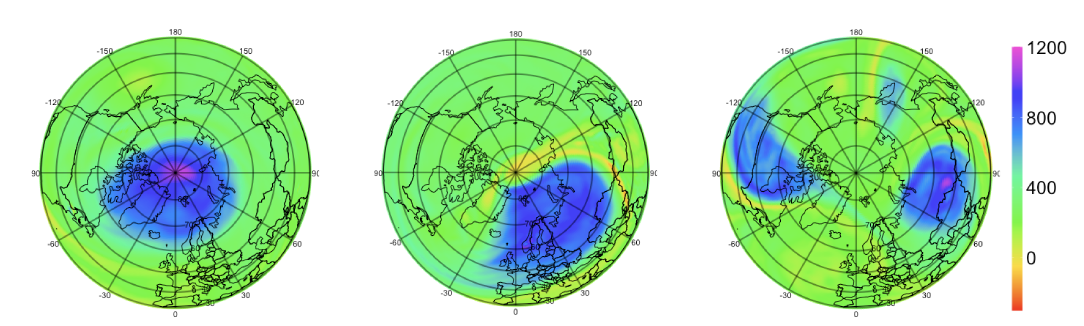
\includegraphics[width=\textwidth]{images/im1.png}
       \label{fig:example_vortex}
       \caption[]{\small Example of potential vorticity of the polar vortex. Undisturbed polar vortex (left) and during two types of SSWs: displacement (middle)
and split (right)~\cite{SlidesRaphael}}
\end{figure}


\newpage
\begin{onecolumn}
\bibliographystyle{IEEEtran}
\bibliography{bibliography}
\end{onecolumn}
	
\end{document}